\section{Date: 2024-10-01}
\noindent \textbf{Series ID: BSCICP035AM665S} 

\noindent This series is titled Composite Leading Indicators: Composite Business Confidence Amplitude Adjusted for Major Five Asia Economies and has a frequency of Monthly. The units are Normalised (Normal=100) and the seasonal adjustment is Seasonally Adjusted.The observation start date is 2000-02-01 and the observation end date is 2023-12-01.The popularity of this series is 4. \\ 

\noindent \textbf{Series ID: CCDIOANYQ156N} 

\noindent This series is titled CredAbility Consumer Distress Index for New York (DISCONTINUED) and has a frequency of Quarterly. The units are Percent and the seasonal adjustment is Not Seasonally Adjusted.The observation start date is 1980-01-01 and the observation end date is 2013-01-01.The popularity of this series is 1. \\ 

\subsection{Regression Tables and Plots}
\begin{center}
\begin{tabular}{lclc}
\toprule
\textbf{Dep. Variable:}               & value\_fred\_CCDIOANYQ156N & \textbf{  R-squared:         } &     0.176   \\
\textbf{Model:}                       &            OLS             & \textbf{  Adj. R-squared:    } &     0.159   \\
\textbf{Method:}                      &       Least Squares        & \textbf{  F-statistic:       } &     10.66   \\
\textbf{Date:}                        &      Tue, 01 Oct 2024      & \textbf{  Prob (F-statistic):} &  0.00198    \\
\textbf{Time:}                        &          14:58:10          & \textbf{  Log-Likelihood:    } &   -154.57   \\
\textbf{No. Observations:}            &               52           & \textbf{  AIC:               } &     313.1   \\
\textbf{Df Residuals:}                &               50           & \textbf{  BIC:               } &     317.0   \\
\textbf{Df Model:}                    &                1           & \textbf{                     } &             \\
\textbf{Covariance Type:}             &         nonrobust          & \textbf{                     } &             \\
\bottomrule
\end{tabular}
\begin{tabular}{lcccccc}
                                      & \textbf{coef} & \textbf{std err} & \textbf{t} & \textbf{P$> |$t$|$} & \textbf{[0.025} & \textbf{0.975]}  \\
\midrule
\textbf{const}                        &     -68.2822  &       44.847     &    -1.523  &         0.134        &     -158.360    &       21.796     \\
\textbf{value\_fred\_BSCICP035AM665S} &       1.4562  &        0.446     &     3.265  &         0.002        &        0.560    &        2.352     \\
\bottomrule
\end{tabular}
\begin{tabular}{lclc}
\textbf{Omnibus:}       &  1.626 & \textbf{  Durbin-Watson:     } &    0.180  \\
\textbf{Prob(Omnibus):} &  0.444 & \textbf{  Jarque-Bera (JB):  } &    1.406  \\
\textbf{Skew:}          & -0.248 & \textbf{  Prob(JB):          } &    0.495  \\
\textbf{Kurtosis:}      &  2.366 & \textbf{  Cond. No.          } & 6.74e+03  \\
\bottomrule
\end{tabular}
%\caption{OLS Regression Results}
\end{center}

Notes: \newline
 [1] Standard Errors assume that the covariance matrix of the errors is correctly specified. \newline
 [2] The condition number is large, 6.74e+03. This might indicate that there are \newline
 strong multicollinearity or other numerical problems.

\begin{figure}
\centering
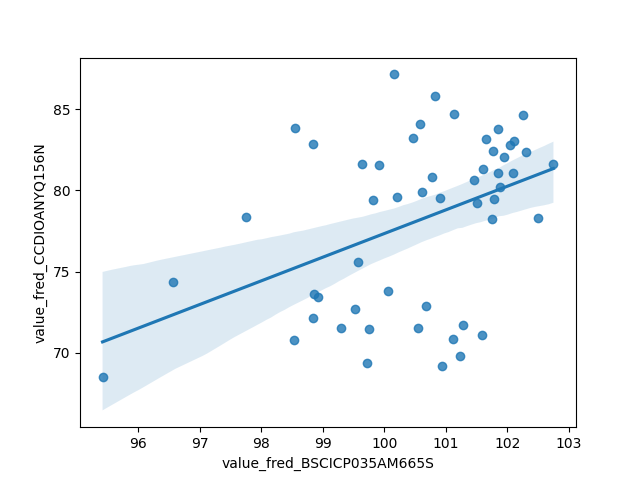
\includegraphics[scale = 0.9]{plots/plot_2024-10-01.png}
\caption{Regression Plot for 2024-10-01}
\end{figure}
\newpage
